\chapter{Results and Analysis}
\label{chap: results}

In this chapter, we will discuss the performance of a two-emulator setup
built using the default configuration of CL: both the massless- and
massive-neutrino emulators appraised here use the COMET priors
(table~\ref{tab: COMET_priors}), $N_k = 300$, and $N_s = 3000$ for both the
training and testing data sets.

The final training LHS had an $s^*$ of 0.07972 in the massive case and 
0.02274 in the massless case. The final testing LHS had an $s^*$ of 0.07275 in 
the massive case and 0.02015 in the massless case. All numbers have been 
rounded to four significant figures.

\section{Quantifying the Performance of the Emulator}

To evaluate the performance of the emulator, we use the testing pipeline
explained in chapters~\ref{chap: emu_outline} and~\ref{chap: implementation}.
That is, we create an LHS of test cosmologies, which the training stages have
never seen, and compare the output of the emulator object to that of
CAMB. As in neural network contexts, GPR performance is typically evaluated
using test sets (\citealp{Mancini}, \citealp{Arico}, and
\citealp{Eggemeier}).\footnote{However, these test sets are
more commonly referred to as ``validation sets.'' We use the phrase
``test set'' to call to mind the three conventional data sets in a machine
learning setup: training, validation, and testing. This distinction will
prove useful in section~\ref{sec: future_work}.}

We appreciate that appraisal based on test sets
may not provide hard boundaries on the true
range of errors associated with the emulators,
because the continuity of the parameter hypervolume means that an infinite
number of cosmologies could be tested. Therefore, traditional
goodness-of-fit tests such as $\chi^2$ do not apply here.
However, precisely because
power spectra vary smoothly in this space\footnote{Indeed, without this
property, interpolation would be unproductive.}, we expect the error 
curves to vary similarly. So long as the test LHS represents a reasonable
coverage of the parameter space, we expect the errors calculated therefrom to
be similarly representative of emulator performance. On the other
hand, at the edges of the parameter space, where interpolation begins to
break down, the errors will be at their highest, and the following analyses
may not be representative of these edge cases.

For this chapter as well as chapter~\ref{chap: disc_and_conc}, we will focus
on just two error metrics: percent error and squared error. We include percent
error as it is more common in the literature and because it is immediately
interpretable (\citealp{Mancini}, \citealp{Arico}, and
\citealp{Eggemeier}). By contrast, the squared errors are difficult to
understand unless compared across multiple similar cases.
Nevertheless, we argue
that squared errors represent a more useful metric, at least within a single
paper, because they are unbiased with respect to the magnitude of the emulated
quantity. Consider that $P(k)$ is smallest at the largest $k$; if an emulator
mispredicts $P(k)$ with a constant offset, then the percent error curves will
be largest at the smallest $k$. As a further example, consider that the
overall amplitude of $P(k)$ is smaller for smaller $\tilde{\sigma}_{12}$;
if we again imagine a constant offset, $\tilde{\sigma}_{12}$ will appear as a
problematic parameter if we look only at percent error.


\section{Percent and Absolute Errors on Random Cosmologies}

\begin{figure}[ht!]
  \centering
  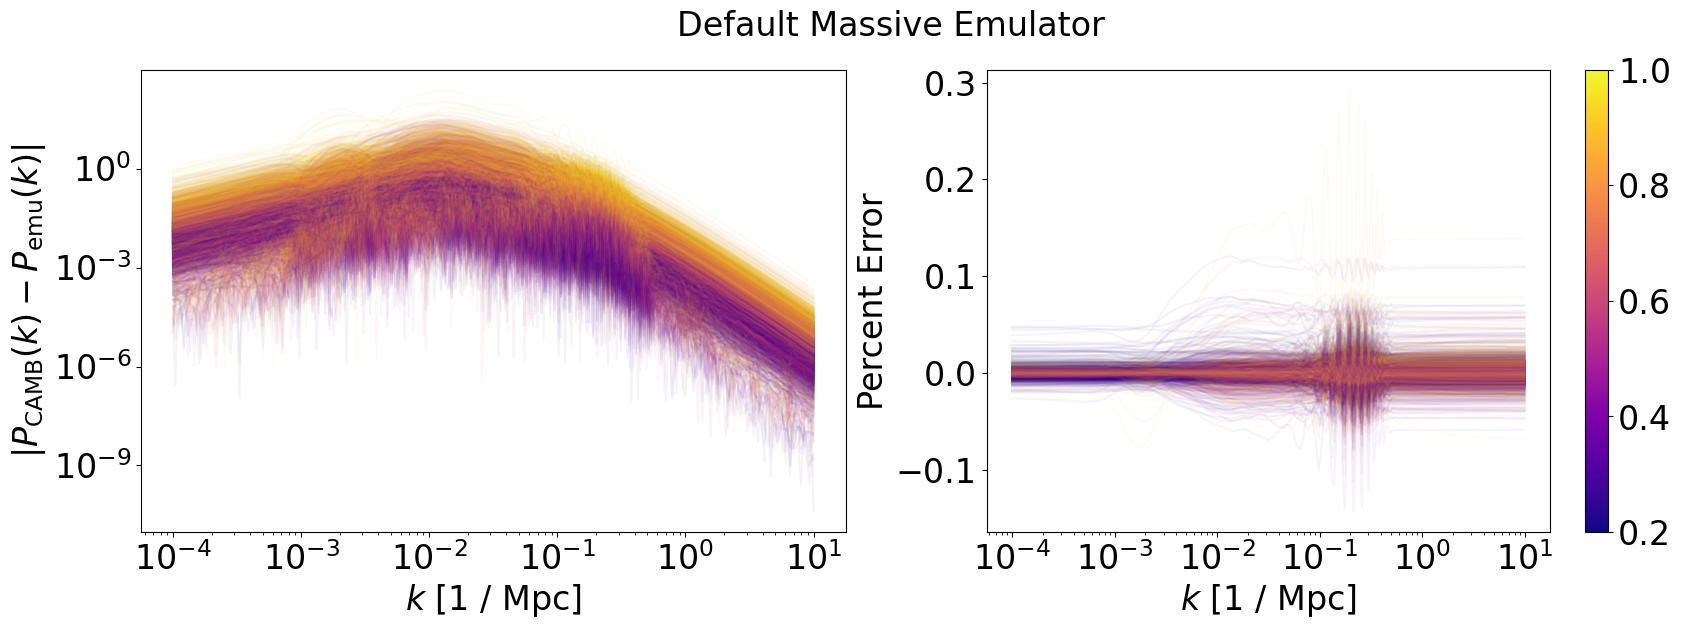
\includegraphics[width=\textwidth]{error_on_emulators/default_massive}
  \caption[Default Massive Emulator Performance]{1000 error curves provided by running the test set through the emulator.}
  \label{fig: def_massive_errs}
\end{figure}

\begin{figure}[ht!]
  \centering
  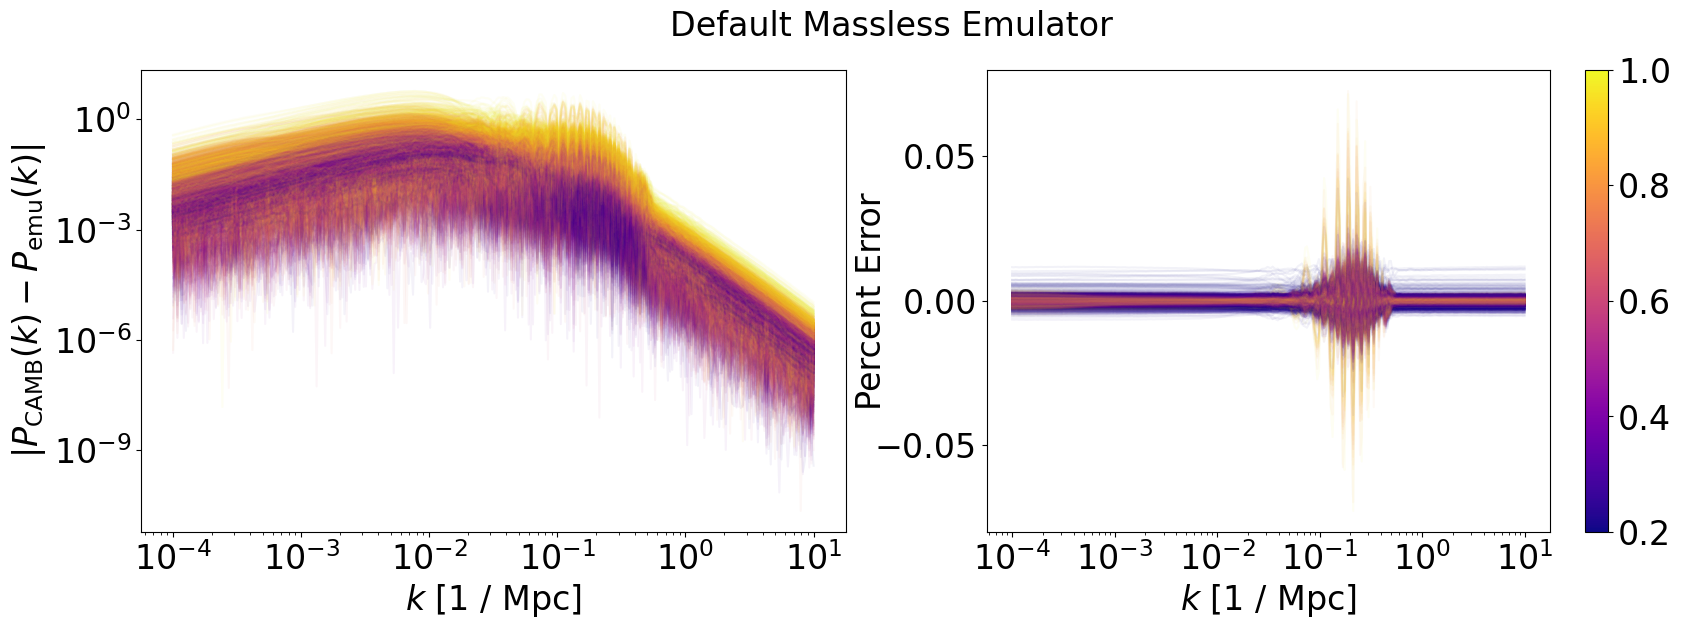
\includegraphics[width=\textwidth]{error_on_emulators/default_massless}
  \caption[Default Massless Emulator Performance]{1000 error curves provided by running the test set through the emulator.}
  \label{fig: def_massless_errs}
\end{figure}


* Percent error curves massless

* Squared error curves massless

* Percent error curves massive

* Squared error curves massive

This will be a fairly short section, basically just showing the plot of 5000 
error curves in these two ways.

\textcolor{orange}{Create some plots focusing on the BAO error spikes? i.e.
zoom-in on k-ranges.}

\textcolor{green}{redo the numbers in this next paragraph}

The current state of the massless-neutrino emulator features sub-0.1\% error 
for the vast majority of scales, with the exception of some wild fluctuations  
between k=0.09 and 0.2 / Mpc. Outside of this range, the errors tend to 
sub-0.01\% in the large-scale regime and sub-0.005\% in the small-scale 
regime. Please refer to figures XXX through XXX for illustrations thereof.

As we can see from figures~\ref{fig: massless_default} 
and~\ref{fig: massive_default}, 
both emulators are most accurate at very large and
very small $k$, with significant difficulties around the BAO region. We
consider the small-scale performance a powerful confirmation of our
techniques, as the impact of massive neutrinos is most significant at small
scales.

We highlight that the massive emulator performs significantly worse than its 
massless counterpart. The emulators are difficult to compare because they
were constructed from LHSs of different dimension: four in the massless case,
six in the massive case. Since $N_s = 5000$ is constant, we expect the 
massless LHS to sample the parameter space much more densely than the massive
LHS. In any case, the discrepancy in accuracies will be worsened by the
approximate nature of our fit from section~\ref{sec: proposed_fit}:
the results of section~\ref{sec: fit_testing} indicate
that evolution parameters besides $A_s$ are necessary for complete
characterization of the impact of massive neutrinos. Nevertheless, the
overall percent error of the massive emulator is \textcolor{green}{nearly}
at the level of CAMB itself, so we consider the massless emulator an
encouraging success.

As evolution-mapping emulation for \textit{massive}-neutrino cosmologies
is the novel feature of this work, we will henceforth concentrate exclusively
on the massive-neutrino emulator.

\textcolor{orange}{I plan to spend some time talking 
about \textit{why} parameter x is the current biggest problem for the 
emulator.}

\textcolor{orange}{It would have been nice if you had done like Andrea said,
and produced a plot colored by the ``extremeness'' of the parameters. We
could implement an extremeness index for parameter $x$ simply by taking
subtracting 0.5 and taking the absolute value, assuming that $x$ comes from
the unit LHS. Then, we could take the average over six parameters to get
an extremeness index for the cosmology as a whole. Optionally, for plot
optimization, you could multiply the final value by 2 so that the extremeness
runs from 0 to 1.}


\section{Improvement from Two-emulator Solution}
\label{sec: 2emu_improvement}

\begin{figure}[ht!]
  \centering
  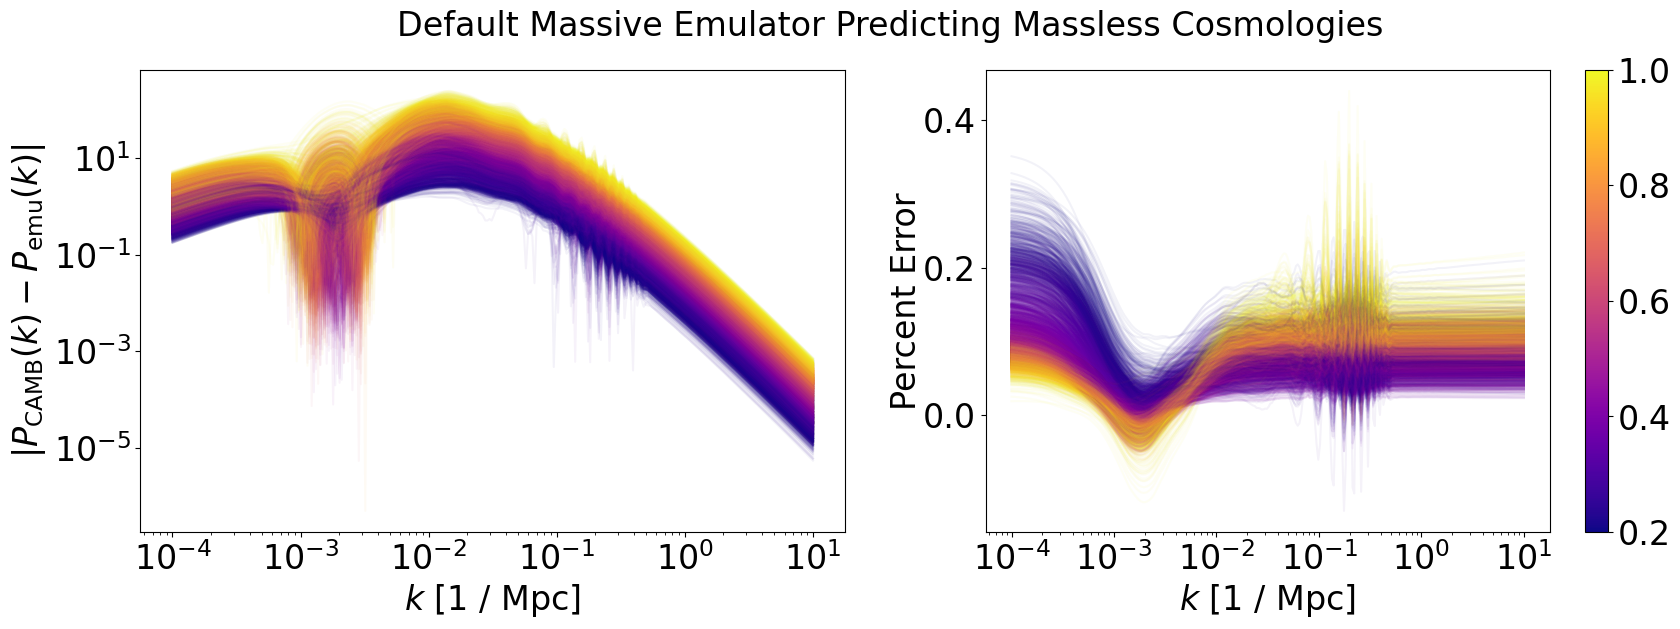
\includegraphics[width=\textwidth]{error_on_emulators/two_emu_improvement}
  \caption[Default Massive Emulator Performance]{1000 error curves provided
  	by running the massless-neutrino test set through the massive-neutrino 
  	emulator. To adjust the four-dimensional massless-neutrino test LHS to
  	the six-dimensional massive-neutrino emulator, we filled in
  	$A_s \approx 2.1272 \cdot 10^{-9}$ and $\omega_\nu = 0$ everywhere.}
  \label{fig: two_emu_errs}
\end{figure}

To justify our use of a two-emulator solution to increase
accuracy in the massless-neutrino case, we task the massive-neutrino emulator with
predictions over the test set of the massless-neutrino emulator. We consider
this a fair test because we sampled $\omega_\nu$ values for the
massive-neutrino emulator from a uniform distribution [0, 0.01]. Therefore,
in principle, the $\omega_\nu = 0$ case should only be a slight extrapolation.

To understand these results, we remind the reader the overall error of the
massive emulator is larger than that of the massless emulator. As mentioned
in 

To justify our decision and to quantify the improvement from this approach, we
have prepared \textcolor{orange}{some} plots in
section~\ref{sec: 2emu_improvement}.

\textcolor{blue}{This will be an extremely short section with some error
plots of the massive-neutrino cosmology evaluating massless-neutrino
cosmologies.}

\section{Minimum Separation of the Training LHC}
\label{sec: error_from_lhc}

What is the impact of the minimum separation? Surely the minimum separation
should be a proxy for the evenness of the coverage of the space of
cosmologies. Therefore, we expect the error variance to increase much more
dramatically than, say, the average bias.

How would we be able to quantify the error due to this? We could try to 
compare the emulator performance trained on hyper cubes of various minimum 
distances.

% The following plots were generated with emu_experiment_histograms.ipynb
\begin{figure}[ht!]
    \begin{subfigure}{0.35 \textheight}
    \centering
 		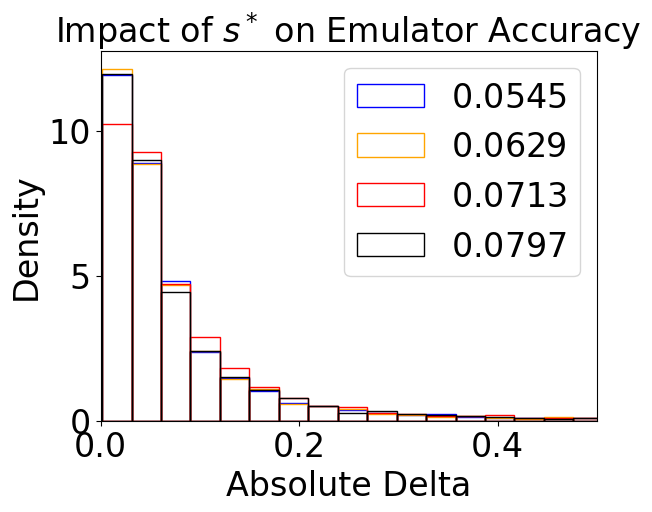
\includegraphics[width=\textwidth]{error_on_emulators/deltas-hist-minsep}
 		\caption{Median absolute errors.}
 		\label{fig: minsep_experiment_deltas}
    \end{subfigure}
    \begin{subfigure}{0.35 \textheight}
    \centering
 		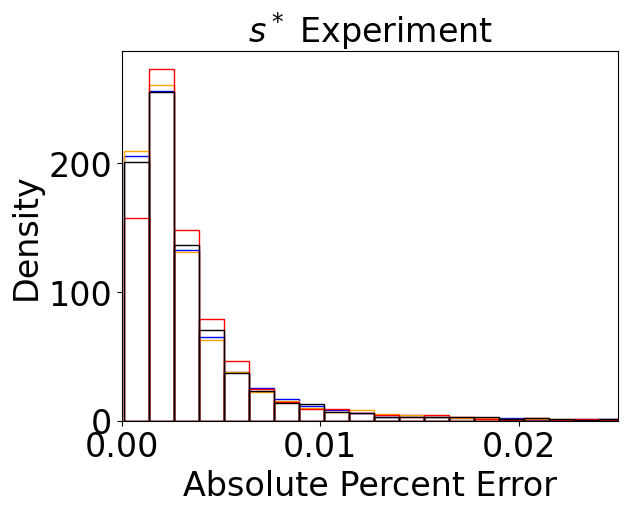
\includegraphics[width=\textwidth]{error_on_emulators/percents-hist-minsep}
 		\caption{Median absolute percent errors.}
 		\label{fig: minsep_experiment_percerr}
    \end{subfigure}
        \centering
    \caption[Impact of $s^*$ on Accuracy]
    		{Histograms of errors associated with emulators trained on LHSs of
    			different $s^*$ values. Doesn't seem to make much difference. For the tested values, see
    			table~\ref{tab:}.}
    \label{fig: minsep_experiment}
\end{figure}

% The following table was generated with emu_experiment_stats.ipynb
\begin{table}[ht!]
\centering
\begin{tabular}{l|l|l|l|l}
\hline
$s^*$ & Median of Means & Median of Medians & Median of STDs & Maximum PTP \\ \hline
$0.0545$ & 0.167753 & 0.045098 & 0.232575 & 205.656917 \\
$0.0629$ & 0.169627 & 0.044320 & 0.234392 & 174.772714 \\
$0.0713$ & 0.194701 & 0.050606 & 0.275545 & 203.590333 \\
$0.0797$ & 0.173023 & 0.044955 & 0.244320 & 224.434379 \\
\end{tabular}
	\cprotect\caption[$s^*$ Experiment: Percent Error Statistics]{The
		results of this experiment are surprising. We consider that there
		may have been an error in our execution of the experiment...}
 \label{tab: minsep_experiment_delta_stats}
\end{table}

% The following table was generated with emu_experiment_stats.ipynb
\begin{table}[ht!]
\centering
\begin{tabular}{l|l|l|l|l}
\hline
$s^*$ & Median of Means & Median of Medians & Median of STDs & Maximum PTP \\ \hline
$0.0545$ & 0.002835 & 0.002240 & 0.002025 & 0.192945 \\
$0.0629$ & 0.002850 & 0.002179 & 0.002079 & 0.196711 \\
$0.0713$ & 0.003052 & 0.002409 & 0.002059 & 0.266151 \\
$0.0797$ & 0.002883 & 0.002255 & 0.002058 & 0.291348 \\
\end{tabular}
	\cprotect\caption[$s^*$ Experiment: Percent Error Statistics]{The
		results of this experiment are surprising. We consider that there
		may have been an error in our execution of the experiment...
		we find it a strange coincidence that the percent errors steadily
		get worse... perhaps the effect is so subtle that we would have to
		run more experiments?}
 \label{tab: minsep_experiment_percerr_stats}
\end{table}

\section{Resolution of the k Axis}

This might go better in the CassL section, but I think I ought to motivate the 
decision to use length-300 arrays.

\begin{figure}[ht!]
  \centering
  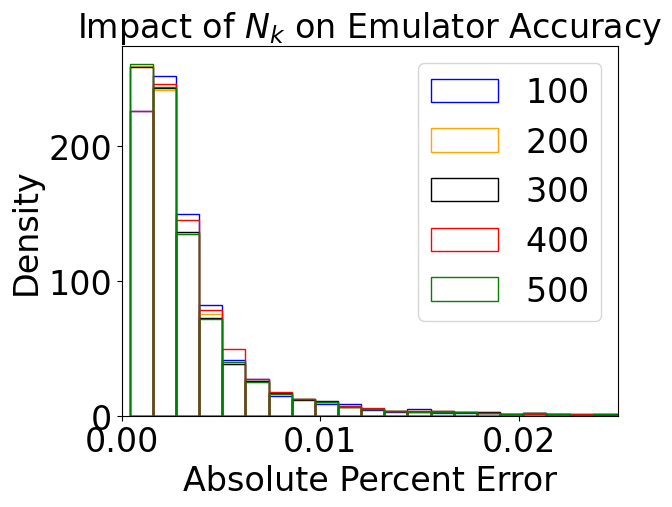
\includegraphics[scale=0.5]{error_on_emulators/percents-hist-N_k}
  \caption[Impact of $N_k$ on Accuracy]{The test is too fair!}
  \label{fig: Nk_experiment}
\end{figure}

This is a special case where we would argue that percent error is more useful 
than squared error.
That is because percent error can be considered on its own, whereas squared
error relies on comparison for its meaning to emerge. But in this case, the
comparisons are obscure. Consider, for example, comparing an $N_k = 100$
emulator with an $N_k = 500$ emulator: the $N_k = 100$ emulator will have
fewer points from which to compute errors. Simple interpolation is not enough
to restore direct comparability, as the $N_k = 500$ emulator by definition
will suffer less from interpolation than the $N_k = 100$ emulator, for which
each point will have to inform five times as much as the interpolated function
domain.

% The following table was generated with emu_experiment_stats.ipynb
\begin{table}[ht!]
\centering
\begin{tabular}{l|l|l|l|l}
\hline
$N_k$ & Median of Means & Median of Medians & Median of STDs & Maximum PTP \\ \hline
$100$ & 0.003082 & 0.002427 & 0.002174 & 0.272042 \\
$200$ & 0.002878 & 0.002243 & 0.002054 & 0.297159 \\
$300$ & 0.002883 & 0.002255 & 0.002058 & 0.291348 \\
$400$ & 0.003034 & 0.002461 & 0.002042 & 0.277015 \\
$500$ & 0.002881 & 0.002221 & 0.002088 & 0.296367 \\
\end{tabular}
	\cprotect\caption[$N_k$ Experiment: Percent Error Statistics]{Caption!}
 \label{tab: Nk_experiment_percerr_stats}
\end{table}

\section{Number of Training Samples}
\label{sec: num_samples}

\textcolor{blue}{Justify choice of 5000 samples for each: maybe we can make a
trend plot showing diminishing returns in test error?}

% The following plots were generated with emu_experiment_histograms.ipynb
\begin{figure}[ht!]
    \begin{subfigure}{0.35 \textheight}
    \centering
 		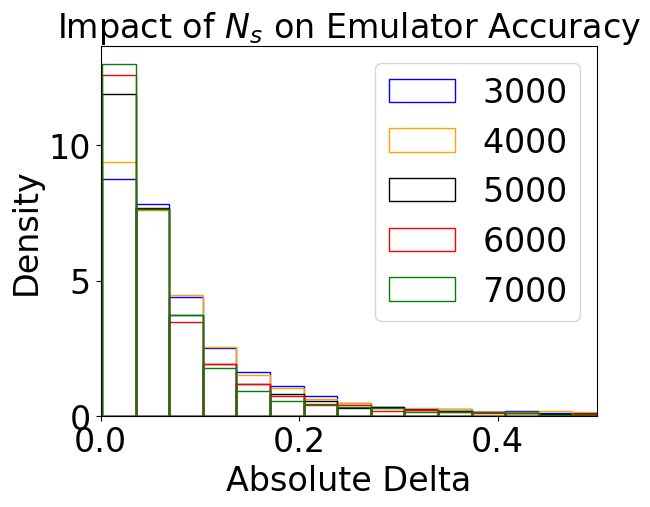
\includegraphics[width=\textwidth]{error_on_emulators/deltas-hist-N_s}
 		\caption{Median absolute errors.}
 		\label{fig: Ns_experiment_deltas}
    \end{subfigure}
    \begin{subfigure}{0.35 \textheight}
    \centering
 		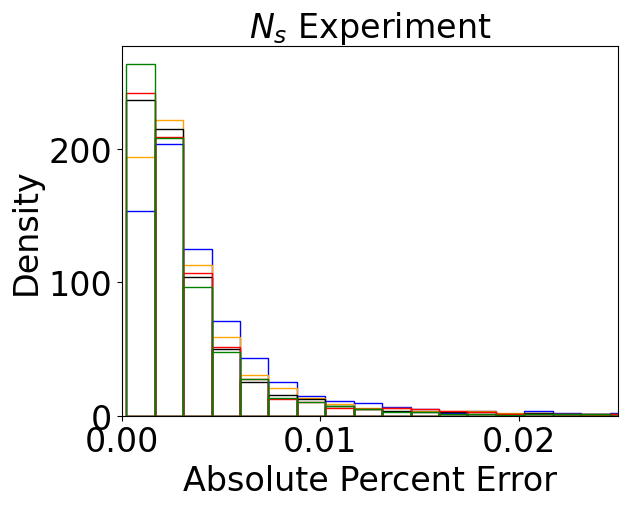
\includegraphics[width=\textwidth]{error_on_emulators/percents-hist-N_s}
 		\caption{Median absolute percent errors.}
 		\label{fig: Ns_experiment_percerr}
    \end{subfigure}
        \centering
    \caption[Impact of $s^*$ on Accuracy]
    		{Histograms of errors associated with emulators trained on LHSs of
    			different $N_s$ values. Doesn't seem to make much difference,
    			but unlike the other cases, we can definitely say here that it
    			makes a difference.}
    \label{fig: Ns_experiment}
\end{figure}

% The following table was generated with emu_experiment_stats.ipynb
\begin{table}[ht!]
\centering
\begin{tabular}{l|l|l|l|l}
\hline
$N_s$ & Median of Means & Median of Medians & Median of STDs & Maximum PTP \\ \hline
$3000$ & 0.2382 & 0.0588 & 0.3388 & 175.5588 \\
$4000$ & 0.2010 & 0.0567 & 0.2741 & 185.5470 \\
$5000$ & 0.1730 & 0.0450 & 0.2443 & 224.4344 \\
$6000$ & 0.1712 & 0.0425 & 0.2415 & 146.6090 \\
$7000$ & 0.1633 & 0.0410 & 0.2305 & 118.7862 \\
\end{tabular}
	\cprotect\caption[$N_s$ Experiment: Deltas Statistics]{Caption!}
 \label{tab: Ns_experiment_deltas_stats}
\end{table}

% The following table was generated with emu_experiment_stats.ipynb
\begin{table}[ht!]
\centering
\begin{tabular}{l|l|l|l|l}
\hline
$N_s$ & Median of Means & Median of Medians & Median of STDs & Maximum PTP \\ \hline
$3000$ & 0.0037 & 0.0030 & 0.0027 & 0.2794 \\
$4000$ & 0.0032 & 0.0026 & 0.0022 & 0.2305 \\
$5000$ & 0.0029 & 0.0023 & 0.0021 & 0.2913 \\
$6000$ & 0.0028 & 0.0022 & 0.0020 & 0.1893 \\
$7000$ & 0.0027 & 0.0021 & 0.0019 & 0.1189 \\
\end{tabular}
	\cprotect\caption[$N_s$ Experiment: Percent Error Statistics]{YES!
		We caution that the last column can be a misleading statistic, but
		it is still a helpful value to quote...}
 \label{tab: Ns_experiment_percerr_stats}
\end{table}


% This might go better in the CassL section, but I think I ought to motivate 
% the decision to use 5000 training arrays.

\textcolor{orange}{I'll have to concede that the results of this section are 
not entirely comprehensive; we didn't train any emulators over the 
uncertainties of analogous validation hypercubes. All comparisons here use the
simpler pipeline of just two data sets, training and testing.}
